\section{Introduction}
\label{intro}
As smart phones penetrate in the world's populations,
applications are increasingly
tracking user locations and offering services based on where the users are or
where they frequently go. Pure latitudes and longitudes provided by GPS
are not useful until they are correlated to specific locations on a map which
carry semantics. These meaningful locations, which are known as
point-of-interests, or POIs, include transport hubs, restaurants,
schools, scenery spots, office buildings, etc. POIs serve as the
basic components in location-based services for exploration and recommendation.
%increasingly interacting between the Internet and GPS services, applications on mobile devices can now obtain users' location and then navigate users to specific destination based on their current location, and users can share their location with their friends on social networks, or search around current location for entertainment spots. To facilitating all above services, the concept of Point Of Interest (POI) is introduced to represent any specific location on a map users maybe interested in, including transport stations, restaurants, schools, outdoor activity places, working places, etc. And POIs serve as the basic components in location-based services for exploration and recommendation.

%In fact, location-based services are becoming more and more popular today, we start to get used to arranging a weekend trip by searching on Yelp for highly rated places, or finding a satisfying restaurant nearby on Foursquare at unfamiliar places.
Ordinary maps provide the names of the POIs only. But not all names are
indicative to the type or category of the POIs, which is extremely useful
information for determining the semantics of the location.
In addition to providing semantics for each POI, categories
naturally group together POIs which are similar to each other
by some common characteristics.
Online map services such as Google Map have started to add
category information for
POIs as tags, often manually labeled by the map provider or the user community.
However, such category tags are far from being complete.
%For better usage of the POIs existed on the map, one of the most important information about a POI is the category it belongs to, without which it couldn't be reached by users who haven't been there before.
For example, Figure \ref{fig:vivo} shows an area in
central Singapore in Google Map.
Some of the POIs are labeled with categories such as ``Food'',
``Shops'' and ``Banks'' (indicated by graphical icons).
Others, such as ``Best Denki'', does not have a label.
Without prior knowledge, it would be hard to know that ``Best Denki''
in Singapore is actually an electronic retailer.
%with several POIs, in case of we are in this area and wish to find an electronic shop, we'd better know ``Best Denki'' is a electronic retailer, which unfortunately not labeled in the map.

Unfortunately, many of category labels are missing in today's maps
or location-based social networks (LBSN).
%Ideally we would like all the POIs have precise categories from the beginning. The reason why some POIs may appear without category labels is that, in order to attract users' participation as well as gain more flexible and user-oriented POIs, location-based social networks often encourage users to add and edit POIs, and during the addition of a POI, category is not an essential entry.
According to the survey from Ye et al. \cite{yemao}, about 30\% POIs in
Whrrl (which is a well-known LBSN) lack category information,
which is a substantial loss of information of the map.

In this paper, we aim to automatically classify POIs on the map of a LBSN
into different categories. In this paper we employ a global classification
hierarchy from Foursquare, showed in Table \ref{tab:Categories},
as the standard categories. This hierarchy provides categories in different
granularity designed for both general needs and specific interests.
For example, ``Best Denki'' will be first classified as ``Shop \& Service'',
which is a first level category identifying its general purpose.
It can be further classified as ``Electronics Store'',
which is a second level category with more details.
Most of the existing proposals consider only
the general first level categories. However, 
a POI may belong to more than one category.
For example many bars offer dinner service as well
which qualifies them as both ``Food'' and ``Nightlife''.
Moreover, according to our experiment,
spatial features also contribute to better performance for
second level categories. 
A standard category hierarchy  works better than
ad hoc labels provided by users. For example, ad hoc labels such as
``restaurant'', ``buffet'', ``cafe'' , ``burger joint'', ``pizza place'',
all belong to the standard ``Food'' category, which avoids confusion.

\begin{figure}[ht]
% Use the relevant command to insert your figure file.
% For example, with the graphicx package use
  \epsfig{file=VenueGraph/vivocityrec.eps,width=\columnwidth}
% figure caption is below the figure
\caption{Vivocity, Singapore (from Google map)}
\label{fig:vivo}       % Give a unique label
\end{figure}

\begin{table}
\caption{1st Level category and Examples of 2rd Level Category}
\label{tab:Categories}
\begin{tabular}{p{4cm}|p{10cm}}
\hline

1st Level Category&	Examples of 2rd Level Category\\
\hline
Arts \& Entertainment&	Aquarium, Art Gallery, Casino, Concert Hall, Movie Theater, Museum, Stadium, Theme Park, Zoo\\
\hline
College \& University&	College Academic Building, College Library, College Residence Hall, College Stadium, Law School, Medical School\\
\hline
Food&	American Restaurant, Buffet, Cafeteria, Chinese Restaurant, Ice Cream Shop, Pizza Place, Tea Room, Wings Joint\\
\hline
Nightlife Spot&	Beach Bar, Beer Garden, Lounge, Karaoke Bar, Sake Bar, Sports Bar\\
\hline
Outdoors \& Recreation&	Athletics \& Sports, Beach, Castle, Farm, Fishing Spot, Forest, National Park, Palace, Ski Area, Vineyard\\
\hline
Professional \& Other Places&	Animal Shelter, Factory, Government Building, Medical Center, Non-Profit, Office, School, Spiritual Center\\
\hline
Residence&	Home (private), Residential Building (Apartment / Condo), Trailer Park\\
\hline
Shop \& Service&	Bank, Bookstore, Car Wash, Clothing Store, Electronics Store, Gym / Fitness Center, Outlet Store, Pet Service, Spa\\
\hline
Travel \& Transport&	Airport, Boat or Ferry, Bus Stop, Hotel, Subway, Taxi, Train Station\\
\hline
\end{tabular}
\end{table}

LBSNs carry not only
names, geographical coordinates, but also users' check-in records.
%Data sources for a POI includes location-based social networks (LBSN), which contains at least the POI's name, users' check-in records, and the location (geographic coordinates) of the POI. Other resources including government diary data \cite{LocationPlacer}, smart phone data \cite{eberle2012mobile}, which provide multi-aspect information from device sensors and manual records. However, the latter resources suffer from privacy problems since they record a single user's trajectory and smart phone logs, and they are difficult to collect and obtain and lack the ability of generalization. In our experiment, we add spatial features into existing features extracted from the former data sources, which comes from LBSN, to show improvement in performance.
We formulate the problem as a supervised multi-label classification problem,
since some of the POIs are labeled with categories by users and some are not.
Then we solve it in a typical classification setting by extracting features
from raw data and use them as input for a classifier, which produces the
category labels.
%In the following, we will focus on the distinctive features
%for each POI.

%Although we start with a rather accessible data sources,
%there are virtually a lot of clues in inferring what category
%a place belongs to based on these information.
The most intuitive features of POIs would be word features extracted
from the names. Besides that, some work, e.g., Ye et al. \cite{yemao},
has focused on the user check-in activities.
They use features based on statistics of user behavior,
including population features (e.g., number of a POI's total check-ins)
and temporal features (e.g., 24-hour distribution of check-in time).
These features turn out to be effective, and are considered BASE features
in this paper as well.
%to start with. There are also some interesting work \cite{userbehavior}
%on analyzing user's check-in behavior though these features
%are not intended to classify POIs, in fact they focus more on
%statistical analysis of user behavior rather than discriminating
%features for classifying POIs.

However, although user behavior is an effective feature,
formulating users' interest profile purely on check-in records is
far-fetched as far as the POI classification problem is concerned.
The reasons are as follows.
First, normal users' check-in frequency is insufficient to make a
reasonable profile of a user's visit preferences,
and there may be very active users who check in a lot but may not check in
to all uncategorized POIs
Second, unlike movie or music, for which user behaviors depend almost
entirely on user interest, the check-in routine of an individual user
is only partly influenced by user's interest,
and probably more by normal life, e.g., working place, shopping places,
restaurants, etc. These are strongly correlated with the activity area of
the user such as where they live or work.
Without differentiating user's real preference and their normal life,
connections between the places introduced by individual users would not
be convincing for POI classification. In other words, POI categories are not
so much distinguished by who visit them, but by {\em how} they are visited,
e.g., time, date and frequency, etc.
% in different categories is not the specific users
%who visit them, since even a food-lover will check-in other places
%than ``Food'' and cannot check in all ``Food'' places he would love
%if he has the chance to be there, but how the users visit them,
%for example the time, date, etc, which expresses more from the POI's angle.
That explains why statistics over large number of users,
such as 24-hour check-in distribution and 7-day check-in distribution turn
out to be more effective in classification according to Ye et al.'s work \cite{yemao}.

%And we believe that it's also the reason why the relatedness
%score between POIs inferred from user-place relationship in Ye. et al's work
%can not help classification on our data.
%Thus, in our work, we use only Ye et al's statistic features (BASE),
%not including the inferred scores.

%During our exploration on this problem,
%we find an interesting aspect of POI that is helpful,
%compensates name features and user behavior features,
%and yields good result as well: spatial information.
In our work, we discover that the spatial aspects of POIs which
has not been considered in the past can potentially complement
the name and user behavior features and thus improve the accuracy of POI
classification.
Although POIs which are close to each other are not necessarily from the same
category, the location of a POI is almost never random
but a deliberate choice when it was established, and it is
heavily influenced by the category of the POI and the neighbors around it.
The following example illustrates why spatial features are useful
when there is insufficient user check-in data and little clue from the
name of the POI. Figure \ref{fig:EgCasa} shows a POI
called ``Casa Bom Vento'' in Singapore. The name is not in English
which is not very useful as far as the word features are concerned.
The place is also not very popular, and has only attracted one check-in record,
which means user behaviors cannot help.
Fortunately, the POI is surrounded by many restaurants, which increases
the odds that it belongs to the ``Food'' category.
%Therefore, with spatial information,
%we conclude ``Casa Bom Vento'' more probable belonging to ``Food''.
POIs in the same categories are gathering together as shown
in Figure \ref{fig:EgCasa}, and tend to have
similar neighborhood. For example, restaurants and shopping malls are
often near each other as shown in Figure \ref{fig:vivo}. 
Moreover, POIs in category other than ``Food'' may have 
other surroundings.
%Apart from above, POIs in the same category
%tend to have similar spatial configurations.
%\KQ{Why do you mean by spatial configurations? what's the difference
%to neighborhood mentioned above?}
For example, ski parks are often alone by themselves as shown in Figure \ref{fig:skipark}.

\begin{figure}[ht]
\begin{minipage}[ht]{0.51\linewidth}
\centering
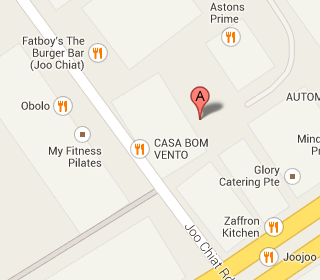
\includegraphics[width=\columnwidth]{VenueGraph/CasaBomVento.PNG}
\caption{Casa Bom Vento, Singapore (from Google map)}
\label{fig:EgCasa}
\end{minipage}
\hspace{0.5cm}
\begin{minipage}[ht]{0.49\linewidth}
\centering
\includegraphics[width=\columnwidth]{VenueGraph/skipark.eps}
\caption{Catfish Bay Water Ski Park, United States (from Google map)}
\label{fig:skipark}
\end{minipage}
\end{figure}

In this paper, we focus on exploring spatial features for POI classification.
We propose a number of spatial features and ways to extract them.
Then, we briefly introduce other features,
including NAME and BASE.
Finally, we show how spatial features complement
the name features and check-in statistics features
to further improve the classification results.
We also conduct experiments on second level classification,
and show stable advantage over the baseline.

Some of the proposed spatial features focus on locations;
while others compute the user behavior statistics of
POIs within certain distance.
These features show different strength and capability in identifying
different categories. We will discuss such difference and fine-tune
the best combination of features for each category.
This paper makes two main contributions:
\begin{itemize}
\item We exploit relative positioning among POIs in combination
with check-in records of users, and
analyze several spatial characteristics in different kinds of POIs;
\item We show spatial features are individually distinctive and effective,
and we manage to produce the best feature combination for each category.
The result outperforms the baseline method using only name features and
user behavior features on real data from Foursquare.
\end{itemize}


